\section{Matrix copy via block reverse ordering}
\textit{Task1} and \textit{Task2} ask for two functions, \texttt{routine1()} and \texttt{routine2()} respectively, that %
take a matrix $M$ of size $N\times N$ and reverse the order in blocks $b\times b$ in another matrix $O$.\\%
As the previous exercise, the only difference between the two functions is whether implicit parallelism is used, %
and I chose again to avoid code duplication and accomplish what was requested via compilation flags.
The compilation commands are the same as used before, adjusted with the new file names. In addition, the \textit{bash} %
script was integrated with the new commands and, as before, each version was executed three times with $b$ values ranging %
from $2^2$ to $2^8$ (inclusive).\\%
Source code \ref{code:matrix} shows the implemented algorithm. It loops around each $b\times b$ block in the original %
matrix $M$ and, for each, copies the values of the current block and the opposite one in the reverse order. Doing both %
copies in the same iteration allows the main matrix to be looped only for half of the rows.
\begin{figure}[h!tb]
    \centering
    \captionsetup{type=plot}
    \caption{\label{plot:matrix}Effective bandwidth by $b$ size}
    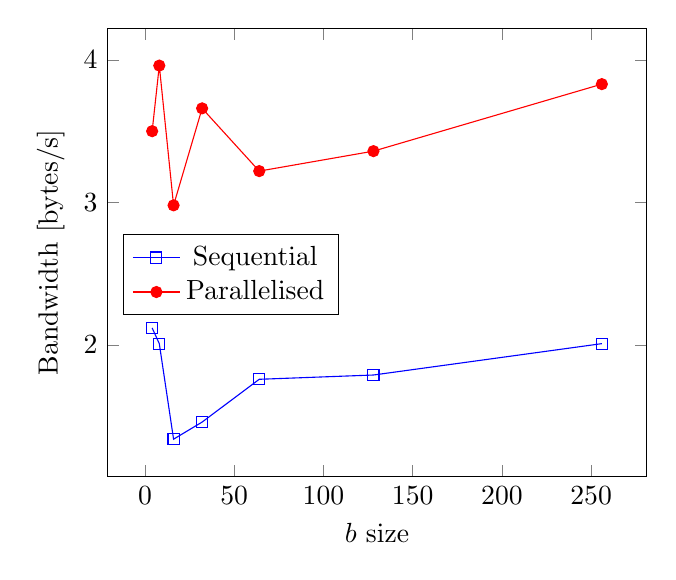
\begin{tikzpicture}
        \begin{axis}[
            title={},
            xlabel={$b$ size},
            ylabel={Bandwidth [bytes/s]},
            legend style={at={(0.03,0.45)},anchor=west}
        ]
            \addplot[
                color=blue,
                mark=square,
                ]
                coordinates {
                    (4,2.12)
                    (8,2.01)
                    (16,1.34)
                    (32,1.46)
                    (64,1.76)
                    (128,1.79)
                    (256,2.01)
                };
            
            \addplot[
                color=red,
                mark=*,
                ]
                coordinates {
                    (4,3.50)
                    (8,3.96)
                    (16,2.98)
                    (32,3.66)
                    (64,3.22)
                    (128,3.36)
                    (256,3.83)
                };
            \legend{Sequential, Parallelised}
        \end{axis}
    \end{tikzpicture}
\end{figure}

\subsection*{Results analysis}
Table \ref{table:matrix_seq} and Table \ref{table:matrix_par} show the run times obtained for each execution. The parallel %
version is 49\% (average) quicker than the same algorithm executed sequentialy.%

\begin{table}[h!tb]
    \centering
    \parbox{.45\linewidth}{
        \centering
\caption{\label{table:matrix_seq}Run times by $b$ size - Sequential (times in seconds)}
\begin{tabular}{@{} c c c c c @{}}
\toprule
    \textbf{Size} & \textbf{Run 1}& \textbf{Run 2}& \textbf{Run 3}& \textbf{Average}\\
\midrule
    $2^2$ & 0.1200 & 0.1300 & 0.1300 & 0.1267\\
\lightrule
    $2^3$ & 0.1400 & 0.1400 & 0.1200 & 0.1333\\
\lightrule
    $2^4$ & 0.2000 & 0.2000 & 0.2000 & 0.2000\\
\lightrule
    $2^5$ & 0.1900 & 0.1700 & 0.1800 & 0.1800\\
\lightrule
    $2^6$ & 0.1600 & 0.1600 & 0.1600 & 0.1600\\
\lightrule
    $2^7$ & 0.1500 & 0.1500 & 0.1500 & 0.1500\\
\lightrule
    $2^8$ & 0.1400 & 0.1300 & 0.1300 & 0.1333\\
\bottomrule
\end{tabular}
%
    }
    \parbox{.50\linewidth}{
        \centering
\caption{\label{table:matrix_par}Run times by $b$ size - Parallelised (times in seconds)}
\begin{tabular}{@{} c c c c c @{}}
\toprule
    \textbf{Size} & \textbf{Run 1}& \textbf{Run 2}& \textbf{Run 3}& \textbf{Average}\\
\midrule
    $2^2$ & 0.0700 & 0.0800 & 0.0800 & 0.0767\\
\lightrule
    $2^3$ & 0.0700 & 0.0600 & 0.0700 & 0.0667\\
\lightrule
    $2^4$ & 0.0800 & 0.1000 & 0.0900 & 0.0900\\
\lightrule
    $2^5$ & 0.0800 & 0.0700 & 0.0700 & 0.0733\\
\lightrule
    $2^6$ & 0.0800 & 0.0900 & 0.0800 & 0.0833\\
\lightrule
    $2^7$ & 0.0700 & 0.0900 & 0.0800 & 0.0800\\
\lightrule
    $2^8$ & 0.0700 & 0.0700 & 0.0700 & 0.0700\\
\bottomrule
\end{tabular}
%
    }
\end{table}

To compute the effective bandwidth, it is necessary to know the number of bytes read $B_r$ and written $B_w$. In our %
case, both values are equal and calculated as $(N\times N) * S_f$, where $N\times N$ is the size of the matrix $M$ and %
$S_f$ is the size of a \textit{float} type (4 bytes). The algorithm reads two values and stores the same %
quantity, totaling four operations for each matrix position. Substituting this information in equation (\ref{eq:bandwidth}), %
we get the results in Table \ref{table:bandwidths}. Plot \ref{plot:matrix} shows a visual representation of the effective %
bandwidth.

\begin{equation}
    \label{eq:bandwidth}
    b=\frac{(B_r+B_w)/10^9}{t}=\frac{(4*4096^2*4)/10^9}{t}\qquad[\textnormal{GB/s}]
\end{equation}

\begin{table}[h!tb]
    \centering
    \caption{\label{table:bandwidths}Effective bandwidths in GB/s}
    \begin{tabular}{@{} c c c @{}}
    \toprule
        \textbf{Size} & \textbf{Sequential}& \textbf{Parallelised}\\
    \midrule
        $2^2$ & 2.12 & 3.50\\
    \lightrule
        $2^3$ & 2.01 & 3.96\\
    \lightrule
        $2^4$ & 1.34 & 2.98\\
    \lightrule
        $2^5$ & 1.49 & 3.66\\
    \lightrule
        $2^6$ & 1.76 & 3.22\\
    \lightrule
        $2^7$ & 1.79 & 3.36\\
    \lightrule
        $2^8$ & 2.01 & 3.83 \\
    \midrule
        Average & 1.79 & 3.50\\
    \bottomrule
    \end{tabular}
\end{table}
\begin{figure}[h!tb]
    \centering
    \captionsetup{type=plot}
    \caption{\label{plot:matrix}Effective bandwidth by $b$ size}
    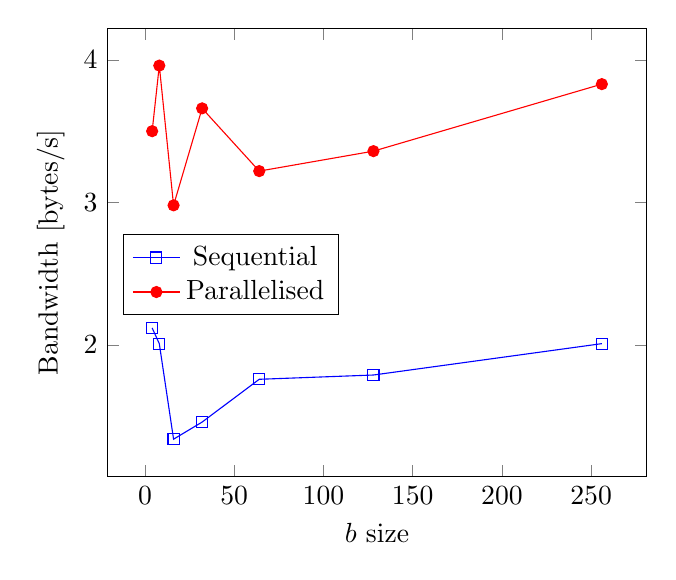
\begin{tikzpicture}
        \begin{axis}[
            title={},
            xlabel={$b$ size},
            ylabel={Bandwidth [bytes/s]},
            legend style={at={(0.03,0.45)},anchor=west}
        ]
            \addplot[
                color=blue,
                mark=square,
                ]
                coordinates {
                    (4,2.12)
                    (8,2.01)
                    (16,1.34)
                    (32,1.46)
                    (64,1.76)
                    (128,1.79)
                    (256,2.01)
                };
            
            \addplot[
                color=red,
                mark=*,
                ]
                coordinates {
                    (4,3.50)
                    (8,3.96)
                    (16,2.98)
                    (32,3.66)
                    (64,3.22)
                    (128,3.36)
                    (256,3.83)
                };
            \legend{Sequential, Parallelised}
        \end{axis}
    \end{tikzpicture}
\end{figure}